
\section{\iris: A Distributed Framework to Support Machine Learning Research}
\label{sec:approach}

This section will present a distributed approach for detecting refactoring commits and calculate software quality metrics before and after each refactoring. Therefore we are using a MapReduce-inspired pattern for data distribution and Apache Spark for pipeline implementation. MapReduce was originally invented by Google and targets big data analysis and calculations by splitting the computation process into a map and a reduce phase \cite{mapreduce2008} on a cluster of computation nodes. Those concepts are reimplemented and available as open source software in Apache Hadoop \cite{hadoop}. Spark improves this pattern by introducing resilient distributed datasets (RDDs) which kept mainly in memory, which results in a faster processing speed than the traditional, hard-drive storage based Hadoop system. Also, Spark allows a better fault tolerance due to directed acyclic graphs (DAGs) for computation tasks. In case one task in the graph fails, Spark can easily restart that specific task without canceling the whole computation.\\

\begin{figure}
\caption{Overview of the refactoring mining pipeline}
\centering
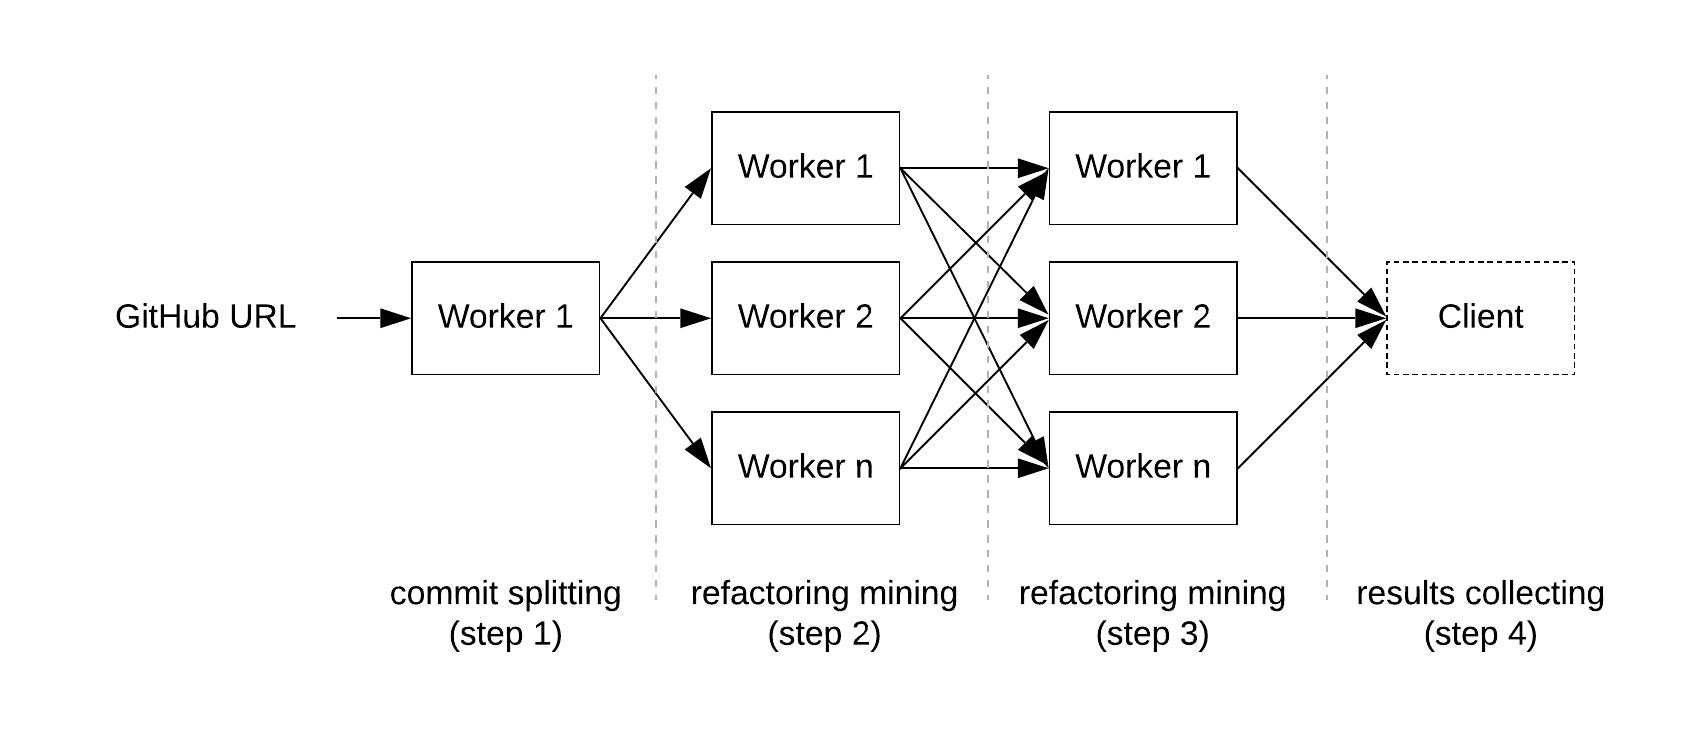
\includegraphics[scale=0.5]{pipeline}
\end{figure}

The pipeline is basically split into three major computation steps: The first step extracts the refactoring operations from a list of given repositories. Spark is cloning one repository instance and scans for commits along the master branch. The list of interesting commits is split into batches of a definable size of \emph{k}-commit and sent by shuffling to each of the other worker nodes.\\
In the second step, each worker starts cloning an separate instance of the repository if does not already exist and runs an instance of RefactoringMiner on the partial list of commits each worker has assigned. The previously described number of \emph{k}-commits depends on the size of memory each worker node has available, as the results are kept in the heap until one batch hash finished the computation. Therefore it is important to adjust \emph{k} accordingly: Is \emph{k} set to high, Spark will fail caused by out of memory exception. Is \emph{k} to small, the performance will decrease as instantiating an instance of RefactoringMiner is an expensive operation. This step outputs a list where each row consists of the repository name, the commit id of the refactoring operation and the type of the refactoring operation (e.g. move method, extract method...). The intermediate results are written as structured data using the Apache Parquet file format \cite{parquet} to reduce storage size and improve performance.\\
The third step takes the shuffled list of refactoring commits identified in the second step and starts again with checking if the repository exists. If not, it gets cloned to that worker node. Now for every batch of refactoring commits an instance of CK is created and the parent commit of the given commit is identified. After that, both commits are checked out and CK calculates the metrics before and after the commit. Additionally, to reduce the computation time and avoid useless data processing, those files that are marked as changed are identified by the Git diff command and the metric calculation is only executed for that list of modified files. As a result, another parquet file is generated containing information about the repository, the involved commits, the refactoring operations (flattened by comma separation), the \emph{side} of the operation (left = commit before refactoring, right = commit after refactoring), the file name, and the metrics.
\subsection{Implementation details}
Both libraries have not been very suitable to fit into our defined in and output format. Therefore they have been forked and slightly modified. RefactoringMiner only provides a method to detect a range of refactoring operations between two commit ids, though it found under certain circumstances more commits than actually existed in this range. Another method that identifies refactoring operations only in one commit was also not suitable in terms of performance and object instantiation. So we added a method that could accept a list of commits without instantiating each time a whole Git repository object. \\
As CK accepts only a source directory, we also forked and modified this library to take a list of interesting files within that directory. That allows the calculation of changed files only within the repository.\\
Besides, the calculation of metrics is designed as abstract metric processors, which improves the simplicity and extensibility of adding custom metric calculation libraries.